\documentclass[10pt,a4paper]{article}
\usepackage[latin1]{inputenc}
\usepackage{amsmath}
\usepackage{amsfonts}
\usepackage{amssymb}
\usepackage{graphicx}
\usepackage{caption}
\usepackage{subcaption}
\usepackage{epstopdf}
\usepackage{subfig}
\usepackage{tabularx}
\bibliography{FEM_ref}
%\usepackage{biblatex}
\title{Finite Element Method Computer Assignment 4.1.1}
\begin{document}

\begin{figure}[t]
	\centering
	
\includegraphics[width=0.5\textwidth]{TU_d_line_P1_color_1.jpg}
\end{figure}

\begin{center}
	\textbf{Computer Assignment 4.1.1}\\
	\textbf{MMP Finite Element Methods (WI4243AP-FE)}
	\begin{tabular}{lr}
		\textbf{Shaikh Bechan} & \textbf{4146425}\\
		\textbf{Zubin Ramlakhan} & \textbf{4170229}\\
	\end{tabular}
\end{center}

\section{Introduction}
The following is a report containing the evaluation of the heat equation with the finite element method.
To solve the two-dimensional heat equation numerically, the finite element method is applied. To that end the minimization problem corresponding to the partial differential in question is derived. The solution of the minimization problem is approximated with the finite element method by deriving the element stiffness matrix and element stiffness vector using triangular and line elements.\\
The code used in the numerical solution can be found in the Appendix.
Please note the theorems and notation are referenced to Numerical Methods in Scientific Computing by J. van Kan, A. Segal, F. Vermolen.

\section{The Heat Equation}
	\begin{figure}[h]
		\centering
		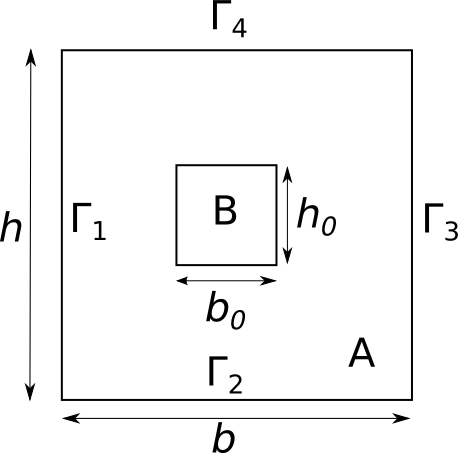
\includegraphics[width=0.6\textwidth]{schem.png}
		\caption{Rectangular plate made of two materials, $A$ and $B$.}
		\label{fig:schem}
	\end{figure}
Consider the rectangular plate shown in figure \ref{fig:schem}, with width $b$ and height $h$. In the center of the plate is a rectangular part, of a different material, with width, $b_0$ and height, $h_0$. $A$ denotes the outer part of the plate while $B$ denotes the inner part.

The situation is stationary and the effects of convection and sources/sinks are absent. Thus the heat equation is simply defined by the conduction (diffusion) term as shown in \eqref{eq:heat}

\begin{equation}\label{eq:heat}
	-\nabla \cdot (k \nabla T) = 0
\end{equation}

with heat conductivity $k$ and temperature $T$. The thermal conductivity is different in each material, i.e. $ k|_A = k_A $ and $k|_B = k_B $.\\

The boundary of $A$, $\partial A$,  is divided in four segments such that $\partial A = \Gamma_1 \cup  \Gamma_2 \cup  \Gamma_3 \cup  \Gamma_4$. On these boundaries the following conditions hold:

\begin{align}
T\rvert_{\Gamma_1\cup\Gamma_3}& = T_0 \label{eq:bc13}\\
\nabla T\rvert_{\Gamma_2} &= 0\label{eq:bc2}\\
k\frac{\partial T}{\partial n}\rvert_{\Gamma_4}=&-\alpha(T_w - T_{\infty})\label{eq:bc4}
\end{align}

In words, the temperature at boundaries $\Gamma_1$ and $\Gamma_3$ are held constant at $T=T_0$. The flux at $\Gamma_2$ is zero. $\Gamma_4$ obeys Newton's heat transfer relation with the thermal diffusivity $\alpha$, the environment temperature $T_{\infty}$ and the temperature at the wall $T_w$.\\

In this problem a symmetry plane is present. This plane runs along the midsection of the plate in the vertical direction. Here, to ensure symmetry, the gradient of the temperature must be zero.

\section{Minimization problem}
A partial differential equation can be related to an equivalent minimization problem with the following theorem:\\

\textbf{Theorem 1 }\textit{Let $L$ be a linear, symmetric, positive differential operator defined of space $\Sigma$ and let}
\begin{equation}\label{eq:pde}
Lu=f
\end{equation}
\textit{Then the solution $u$ minimizes the functional}
\begin{equation}\label{eq:min}
I(u) = \underset{\Omega}{\int}\{\frac{1}{2}uLu-uf\}d\Omega
\end{equation}  \textit{over the space $\Sigma$. On the other hand, if $u$ minimizes \eqref{eq:min} then $u$ satisfies \eqref{eq:pde}} \\

Another requirement $u$ should obey is homogeneous boundary conditions, a requirement $T$ fails. Even so, this theorem can still be utilized by making the boundary conditions homogeneous.

Let $Lu=f$ with non-homogeneous boundary equations and suppose that there is another smooth function $w$ that also satisfies the same non-homogeneous boundary conditions. Now let 
\begin{equation}\label{eq:v}
v=T-w
\end{equation}
$T$ and $w$ satisfy the same non-homogeneous boundary conditions, therefore $v$ satisfies homogeneous boundary conditions. Now the theorem can be applied to $v$ as it meets all the requirements. \\

\begin{equation}\label{rhsv}
Lv=LT-Lw=f-Lw
\end{equation}
so the corresponding minimization problem is given by 

\begin{equation}\label{eq:min1}
\underset{v\in\Sigma} {min}I(v) = \frac{1}{2}\underset{\Omega}{\int}vLvd\Omega-\underset{\Omega}{\int}v(f-Lw)d\Omega
\end{equation}

Substituting \eqref{eq:v} into \eqref{eq:min1} yields

\begin{equation}\label{eq:min2}
\underset{v\in\Sigma} {min}I(v) = \frac{1}{2}\underset{\Omega}{\int}(T-w)L(T-w)d\Omega-\underset{\Omega}{\int}(T-w)(f-Lw)d\Omega
\end{equation}

$f=0$ and $L = -\nabla\cdot( k\nabla)$ according to \eqref{eq:heat}, so \eqref{eq:min2} is rewritten as

\begin{equation}\label{eq:min3}
	\begin{split}
	\underset{v\in\Sigma} {min}I(v) & = -\frac{1}{2}\underset{\Omega}{\int}(T-w)\nabla\cdot(k\nabla(T+w))d\Omega\\
	&=\frac{1}{2}\underset{\Omega}{\int}\nabla (T-w)(k\nabla(T+w))-\nabla\cdot\{(T-w)(k\nabla(T+w))\}d\Omega\\
	&=\frac{1}{2}\underset{\Omega}{\int}\nabla (T-w)(k\nabla(T+w))d\Omega - \frac{1}{2}\underset{\Gamma}{\int}(T-w)(k\nabla(T+w))\cdot\textbf{\^{n}} d\Gamma\\
	&=\frac{1}{2}\underset{\Omega}{\int}\nabla T\cdot k \nabla T d\Omega - \frac{1}{2}\underset{\Omega}{\int}\nabla w\cdot k \nabla w d\Omega\\  &-\frac{1}{2}\underset{\Gamma}{\int}(T-w)(k\nabla(T+w))\cdot\textbf{\^{n}} d\Gamma
	\end{split}
\end{equation}
where the product rule and subsequent Gauss theorem is applied to expand the integral in two volume integrals and one boundary integral. The second integral is independent of $T$ and thus has no influence on the minimization and can be neglected. \\

The boundary integral is evaluated over four boundaries by taking in account the boundary conditions \eqref{eq:bc13}$-$\eqref{eq:bc4}. 

\begin{align}\label{eq:bcint13}
	\frac{1}{2}\underset{\Gamma_1\cup\Gamma_3}{\int}(T_0-T_0)(k\nabla(T+w))\cdot\textbf{\^{n}} d\Gamma &= 0\\
	\frac{1}{2}\underset{\Gamma_2}{\int}(T-w)(k(0+0))\cdot\textbf{\^{n}} d\Gamma & = 0\label{eq:bcint2}\\ 
	\frac{1}{2}\underset{\Gamma_4}{\int}(T-w)(k\nabla(T+w))\cdot\textbf{\^{n}} d\Gamma & = \frac{1}{2}\underset{\Gamma_4}{\int}Tk\frac{\partial T}{\partial n}d\Gamma - \frac{1}{2}\underset{\Gamma_4}{\int}wk\frac{\partial w}{\partial n}d\Gamma\nonumber\\
	&=-\frac{1}{2}\underset{\Gamma_4}{\int}\alpha T(T_w-T_{\infty})d\Gamma \label{eq:bcint4}
\end{align}
where $\frac{1}{2}\underset{\Gamma_4}{\int}wk\frac{\partial w}{\partial n}d\Gamma$ in \eqref{eq:bcint4} is neglected as it too is independent of $T$.\\

Finally, the general minimization problem is given by
\begin{equation}\label{eq:minf}
\underset{T\in\Sigma} {min }I(v) =\frac{1}{2}\underset{\Omega}{\int}k\lvert\nabla T \rvert ^{2}  d\Omega + \frac{1}{2}\underset{\Gamma_4}{\int}\alpha T(T_w-T_{\infty})d\Gamma 
\end{equation}
with $\Sigma: \{T\rvert\quad T\rvert_{\Gamma_1\cup\Gamma_3}=T_0\}$. The boundary conditions \eqref{eq:bc13} and \eqref{eq:bc2} are essential boundary conditions.
% % insert part regarding continuity at interface.

\section{Element stiffness matrix and element stiffness vector}
This problem can be solved by computing the element stiffness matrix and the element stiffness vector.
To do this, the solution is approximated with piecewise linear functions $\phi_j(x,y)$ such that

\begin{equation}\label{eq:app}
T(x,y) \simeq T^n (x,y) =\displaystyle\sum^n_{j=1} c_j \phi_j(x,y)
\end{equation}

One might derive the matrix and vector by substituting this approximation into the minimization problem $\underset{T\in\Sigma} {min}I(v) $ and then set the derivative of $c_j$ to zero. This is called the Ritz method.\\

The second method is by deriving the Galerkin equations. To that end the partial differential equation is multiplied with a test function $\phi$ to derive these equations. Afterwards the approximation of the solution is substituted into the weak form which then results in the element stiffness matrix and element stiffness vector. \\

Both methods yield the same results. The following shows how the matrix and vector are acquired using Galerkin's method. First, the Galerkin equations:

\begin{align}\label{eq:Gal1}
-\underset{\Omega}{\int}\phi \nabla \cdot(k\nabla T)d\Omega&=0\nonumber\\
-\underset{\Omega}{\int} \nabla \cdot \left(\phi k \nabla T\right)- \nabla \phi k \nabla Td\Omega &=0\nonumber\\
-\underset{\Gamma}{\int}\phi k \frac{\partial T}{\partial n} d\Gamma + \underset{\Omega}{\int}\nabla \phi k \nabla Td\Omega &=0\nonumber\\
\underset{\Gamma_4}{\int}\phi \alpha \left(T_w -T_{\infty}\right)d\Gamma + \underset{\Omega}{\int}\nabla \phi k \nabla T d\Omega&=0
\end{align}

where the boundary integral in the penultimate line is split up over the four boundaries like in \eqref{eq:bcint13} - \eqref{eq:bcint4} yielding \eqref{eq:Gal1} as a result. \\

The weak form is thus formulated as follows:
\begin{equation*}
\underset{\Gamma_4}{\int}\phi \alpha \left(T_w -T_{\infty}\right)d\Gamma + \underset{\Omega}{\int}\nabla \phi k \nabla T d\Omega=0
\end{equation*}
$\textit{Find } T\in \Sigma\{\textit{T sufficiently smooth } \rvert T_{\Gamma_1 \cup \Gamma_3 }=T_0\}, \forall \phi \in \Sigma$\\

Now the approximation \eqref{eq:app} is applied. $\phi$ is approximated in the same way i.e.

\begin{equation*}
\phi \simeq \displaystyle\sum^n_{i=1} b_i \phi_i = \phi_i, i=1...n 
\end{equation*}
As $\phi$ is chosen arbitrarily, it is useful to make one of the of the coefficients $b_i$ equal to one and the others to zero.\\

Substituting these approximations into the weak form results in 
\begin{align}\label{eq:weakapp}
\underset{\Gamma_4}{\int} \alpha \phi_i  \left(\displaystyle\sum^n_{j=1} c_j \phi_j - T_{\infty}\right)d\Gamma + \underset{\Omega}{\int}\nabla \phi_i k \nabla \displaystyle\sum^n_{j=1} c_j \phi_j d\Omega &=0\nonumber\\
\displaystyle\sum^n_{j=1} c_j \cdot \alpha\underset{\Gamma_4}{\int}  \phi_i  \phi_jd\Gamma + \displaystyle\sum^n_{j=1} c_j \cdot \underset{\Omega}{\int}\nabla \phi_i k \nabla  \phi_j d\Omega &= \displaystyle\sum^n_{j=1} c_j\cdot \alpha\underset{\Gamma_4}{\int} \phi_i T_{\infty}d\Gamma \\
&(i=1...n)\nonumber
\end{align}

\eqref{eq:weakapp} can be written more compactly as 
\begin{equation*}
\displaystyle\sum^n_{j=1} c_j S_{ij} = f_i
\end{equation*}

with the element stiffness vector 

\begin{equation*}
f_i =\alpha\underset{\Gamma_4}{\int} \phi_i T_{\infty}d\Gamma 
\end{equation*}

and the element stiffness matrix that consists of a boundary matrix 

\begin{equation*}
S^{B}_{ij} = \alpha\underset{\Gamma_4}{\int}  \phi_i  \phi_jd\Gamma 
\end{equation*}

 and a volume matrix
 
\begin{equation*}
 S^V_{ij} = \underset{\Omega}{\int}k\nabla \phi_i  \nabla  \phi_j d\Omega
\end{equation*}
 
The matrices and vector need to be evaluated and are done so using the theorem of  Holland \& Bell .\\

\textbf{Theorem 2 Holland \& Bell} \textit{Let S be a simplex in $\mathbb{R}$ and let $\Delta$ be the determinant defined by }

\begin{equation*}\label{eq:det1}
\Delta = \begin{vmatrix}
1		& x^1_{0} 		& x^1_{2} 		& \dots 	& x^1_{n}\\
1		& x^2_{0} 		& x^2_{2} 		& \dots 	& x^2_{n}\\
\vdots	& \vdots		& \vdots 		& \vdots	& \vdots \\
1		& x^{n+1}_{0} 	& x^{n+1}_{2} 	& \dots 	& x^{n+1}_{n}
\end{vmatrix}
\end{equation*}
\textit{with} \textbf{x}$^1$, \textbf{x}$^2$, $\cdots$ \textbf{x}$^{n+1}$ \textit{the vertices of S.}\\

\textit{Let} $\lambda_i$(\textbf{x}) \textit{be the linear basis functions over S defined by}

\begin{equation*}
\begin{split}
\lambda_i(\textbf{x}) \quad& \textit{ linear}\\
\lambda_i(\textbf{x}^j)=\delta_{ij} \quad& i,j=1,2\cdots n+1
\end{split}
\end{equation*}
\\
\textit{Then the following general integration rule holds:}

\begin{equation*}
\underset{S}{\int}\lambda^{m_1}_1\lambda^{m_2}_2\cdots \lambda^{m_{n+1}}_{n+1}d\Omega = \frac{m_1! m_2! \cdots m_{n+1}!}{\left(\underset{i}{\Sigma} \, m_i +n \right)! }\lvert \Delta \rvert,
\end{equation*}
\textit{for all} $m_i\geq 0$.\\

$\underset{i}{\Sigma} \, m_i$ represents the dimensionality of the elemeng i.e. 2 for triangular elements and 1 for line elements.\\

The set of functions $\phi_i $ are piecewise linear functions and therefore can be written as 
\begin{equation*}
\phi_i = \alpha_i + \beta_i x +  \gamma_i y
\end{equation*}

The determinant of these basis functions are equal to 
\begin{equation*}\label{eq:det2}
\Delta = \begin{vmatrix}
1		& x^1 		& y^1\\
1		& x^2 		& y^2\\
1		& x^3 		& y^3
\end{vmatrix}
\end{equation*}

which is equal to twice the area of a triangular element.\\


According to Holland \& Bell, $f_i$ is evaluated as follows:
\begin{align}\label{f}
f_i &=\alpha T_{\infty}\underset{\Gamma_4}{\int}  \phi_i d\Gamma \nonumber\\ 
    &= \alpha T_{\infty}\rVert\textbf{x}_{l1}-\textbf{x}_{l2}\rVert\frac{1!}{(1+1)!}\nonumber\\ 
    &=  \frac{1}{2} \alpha T_{\infty}\rVert\textbf{x}_{l1}-\textbf{x}_{l2}\rVert
\end{align}
In this case, the integral is a boundary integral. Therefore, the elements along that boundary are one dimensional line elements with dimensionality 1. Hence instead of a determinant, the length $\rVert\textbf{x}_{l1}-\textbf{x}_{l2}\rVert$ of one element is needed.\\
 
$ S^B_{ij} $ is evaluated in almost the same way. The difference is that a distinction between the cases $i=j$ and $i\neq j$ is need as seen in \eqref{eq:SB}
 
 \begin{equation}\label{eq:SB}
 S^{B}_{ij} = \alpha\underset{\Gamma_4}{\int}  \phi_i  \phi_jd\Gamma  = \alpha \lVert \textbf{x}_{l1}-\textbf{x}_{l2}\rVert\cdot \begin{cases}
 \frac{2!0!}{(1+2+0)!} = \frac{1}{3} & i =j\\
 \frac{1!1!}{(1+1+1)!} = \frac{1}{6} & i \neq j
 \end{cases}
 \end{equation}
\\

Before 	\textbf{theorem 2} is applied to $S^V_{ij}$ the gradients of the basis functions are rewritten as 

\begin{equation*}
\nabla \phi_i  \nabla  \phi_j = \left(\beta_i \beta_j+\gamma_i \gamma_j\right) 
\end{equation*}
\\
This value is a constant and can be put in front of the  integral. $S^V_{ij}$ is equal to
\begin{equation}
 S^V_{ij} = k  \left(\beta_i \beta_j+\gamma_i \gamma_j\right)\underset{\Omega}{\int} d\Omega =k  \left(\beta_i \beta_j+\gamma_i \gamma_j\right)\frac{\lVert\Delta\rVert}{2}
\end{equation}

The integral is essential the surface of the triangular element which is equal to half the determinant. \\
The plate can have two values for $k$ depending on the elements being on area A or area B. Therefore $S^V_{ij}$ must change accordingly i.e. $k$ must assume the value corresponding to the material where the elements are situated.

\section{Computation}
\subsection{Mesh}
Before computing the element stiffness matrix and vector, a mesh has to be created. This mesh consists of a grid of triangular elements along the surface of the plates and line elements on the boundaries.\\

The data specific to the problem is given in table \ref{table:dim}.

\begin{table}\label{tabel:dim}
\begin{center}

\begin{tabular}{cccccc}
$T_0$ & = & 1 & $h_0$ & = & 0.4\\
$k_A $ & =& 0.1 & $h$ & =&1\\
$k_B$ & = & 1\\
$\alpha$ & = & 0.01 & $b_0$ & = &0.4\\
$T_{\infty}$ &= & 0 & $b$ &=& 1
\end{tabular} 
\end{center}
\caption{Dimensions of the plate and other parameters.}
\label{table:dim}
\end{table}


The problem is symmetrical along the $y$-axis, therefore the computational effort can be reduced by generating a mesh that covers half the domain. Such a mesh can be seen in the figure %\ref{mesh}
%insert picture mesh
\subsection{Results}
Due to the boundary conditions, the solution is expected to portray some sort of cooling at the top of the plate. The sides remain the same temperature, while the insulation at the bottom requires the isotherms to cross the plate perpendicular. \\


Figure \ref{fig:001} displays the problem's solution with increasing numbers of elements and at $\alpha = 0.01$ in the form of contour plots and color plots. The solution indeed behaves as predicted. The color bars next to the color plots confirm that the temperature of the plate never exceeds the temperature of the side and is positive everywhere, ruling out nonphysical behavior. The temperature is continuous is also across the interface of the two plates as expected.
Also noticeable is the effect of the increase of elements. A rough mesh can lead to some crooked behavior in the isotherms. A finer mesh has a smoothing effect on this crookedness. Looking at the results, a mesh of 50 elements horizontal and vertical seems to suffice at yielding a trustworthy numerical solution to the heat equation.\\

The same problem is redone for a different value of $\alpha$ i.e. $\alpha = 10$, the result of which can be seen in figure \ref{fig:10}. The overall profile of the isotherms remains the same, but the crucial difference is the fact that, due to the larger value of $\alpha$, the cooling effect is much larger. That can be noticed from the fact that the cooling effect has penetrated the plate much further when figure \ref{fig:10} is compared to figure \ref{fig:001}.\\
Again, the increase in number of elements has a smoothing effect, but like with the lower value for $\alpha$, around 50 elements in both directions suffices.

\begin{figure}[h]
\centering
        \begin{subfigure}[b]{0.45\textwidth}
                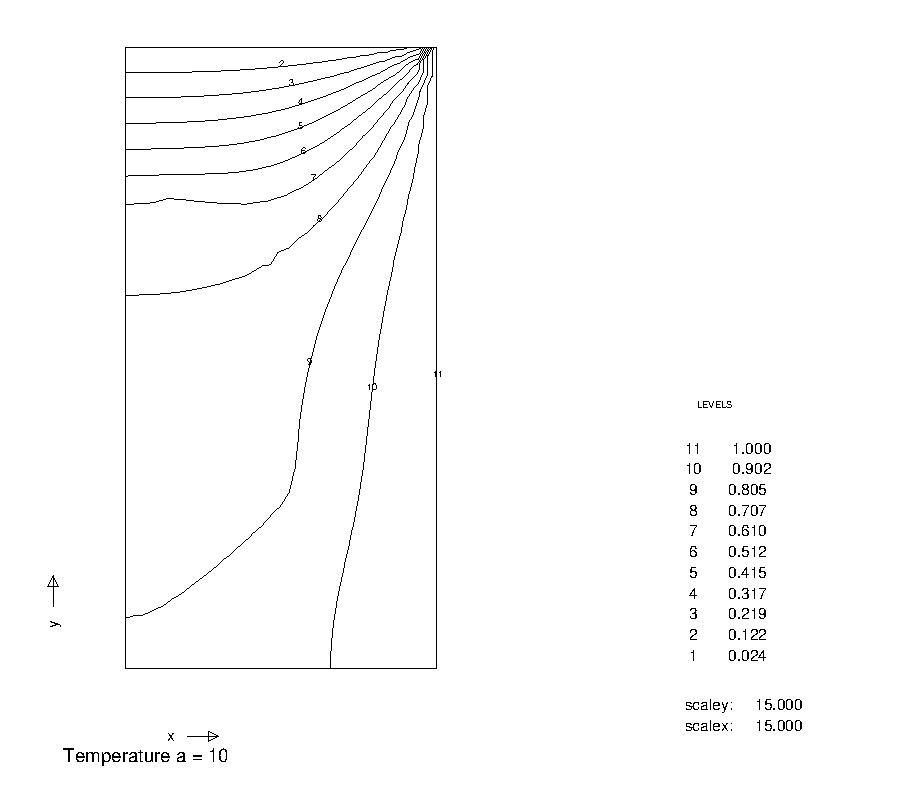
\includegraphics[width=\textwidth]{cont_a10_20el}
                \caption{20 elements contour plot}
                \label{fig:cont_a10_20el}
        \end{subfigure}
        ~
        \begin{subfigure}[b]{0.45\textwidth}
                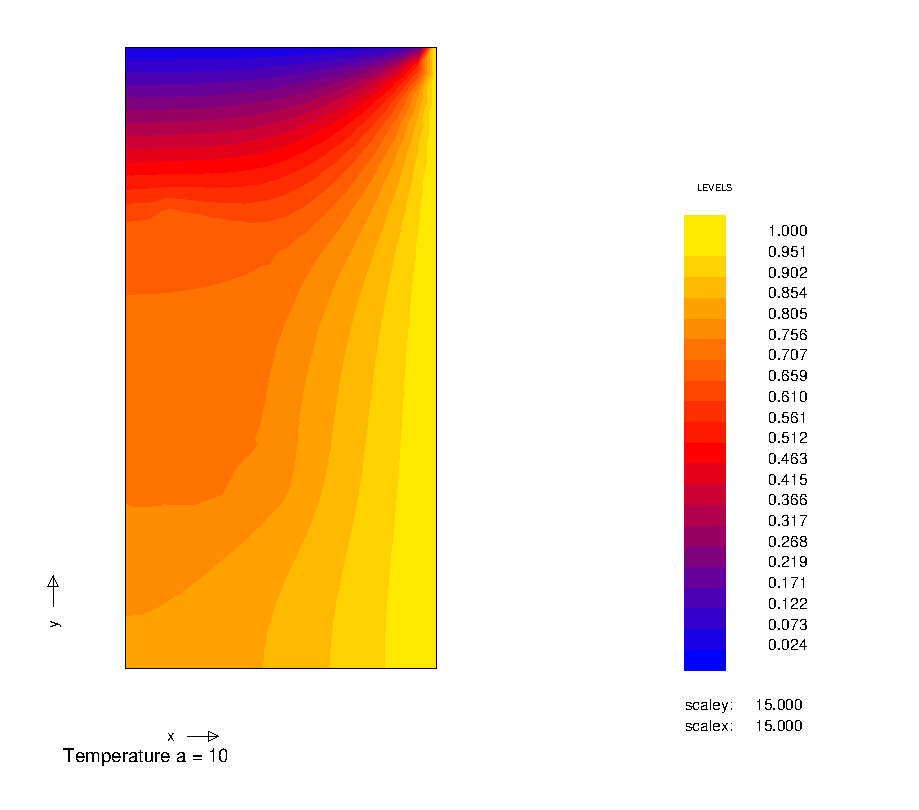
\includegraphics[width=\textwidth]{colplot_a10_20el}
                \caption{20 elements color plot}
                \label{fig:colplot_a10_20el}
        \end{subfigure}
        ~           
        \begin{subfigure}[b]{0.45\textwidth}
                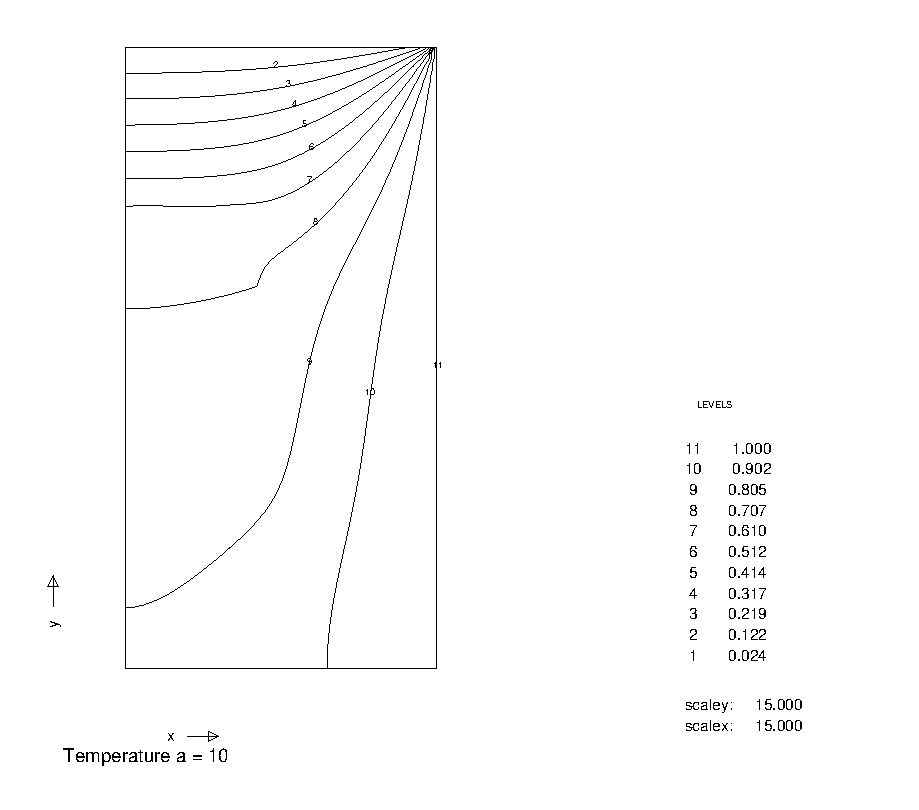
\includegraphics[width=\textwidth]{cont_a10_50el}
                \caption{50 elements contour plot}
                \label{fig:col_a10_50el}
        \end{subfigure}      
        ~
        \begin{subfigure}[b]{0.45\textwidth}
                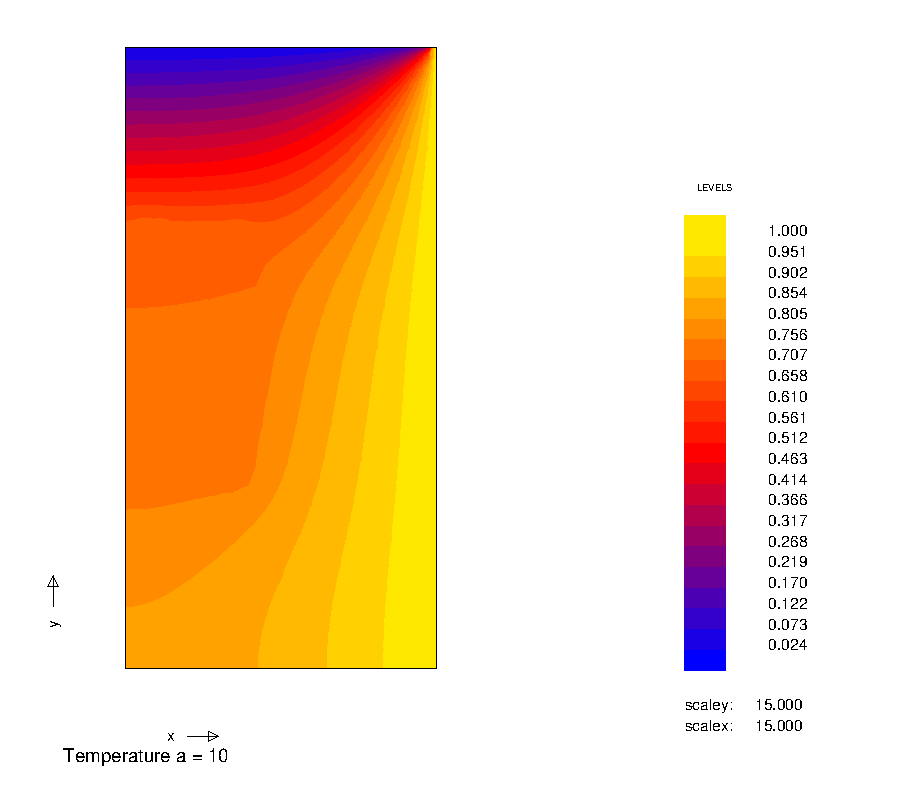
\includegraphics[width=\textwidth]{colplot_a10_50el}
                \caption{20 elements color plot}
                \label{fig:colplot_a10_50el}
        \end{subfigure}
        ~
        \begin{subfigure}[b]{0.45\textwidth}
                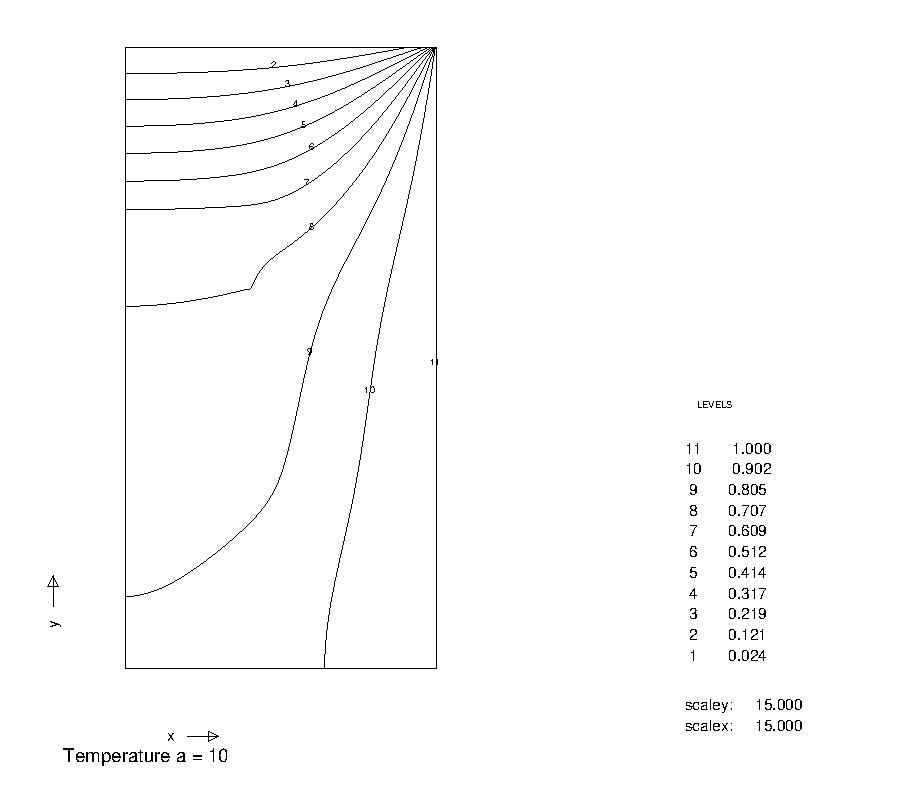
\includegraphics[width=\textwidth]{cont_a10_99el}
                \caption{99 elements contour plot}
                \label{fig:cont_a10_99el}
        \end{subfigure}
        ~ 
        \begin{subfigure}[b]{0.45\textwidth}
                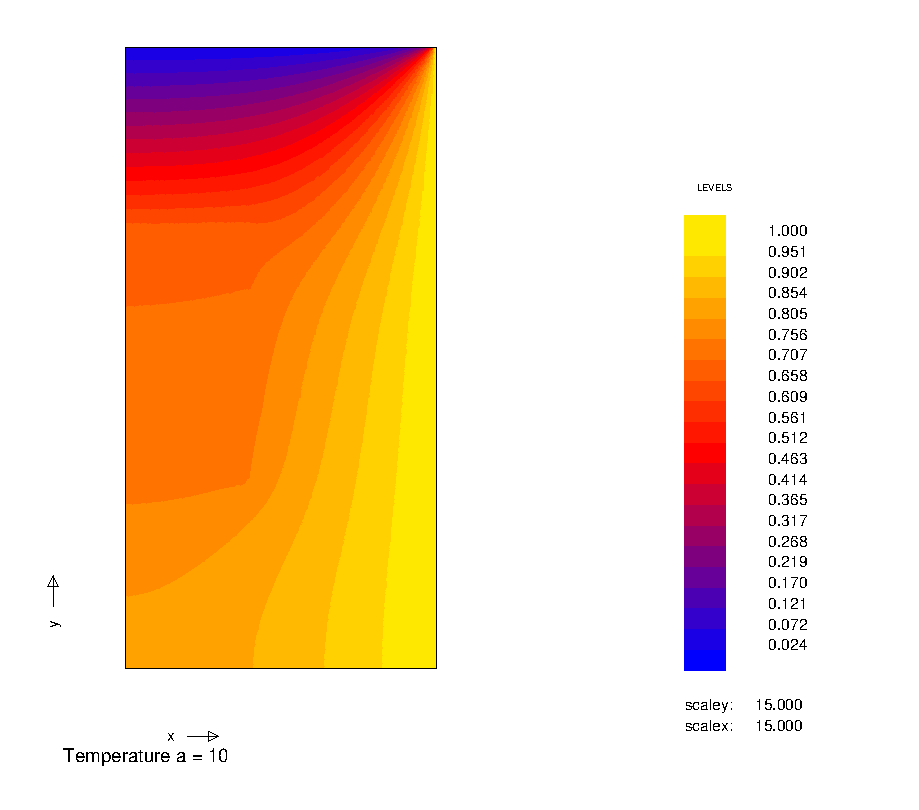
\includegraphics[width=\textwidth]{colplot_a10_99el}
                \caption{99 elements color plot}
                \label{fig:colplot_a10_99el}
        \end{subfigure}
        \caption{solution of the heat equation for a number of elements with $\alpha = 0.01$} 
        \label{fig:001}                                
\end{figure}

\begin{figure}[h]
\centering
        \begin{subfigure}[b]{0.45\textwidth}
                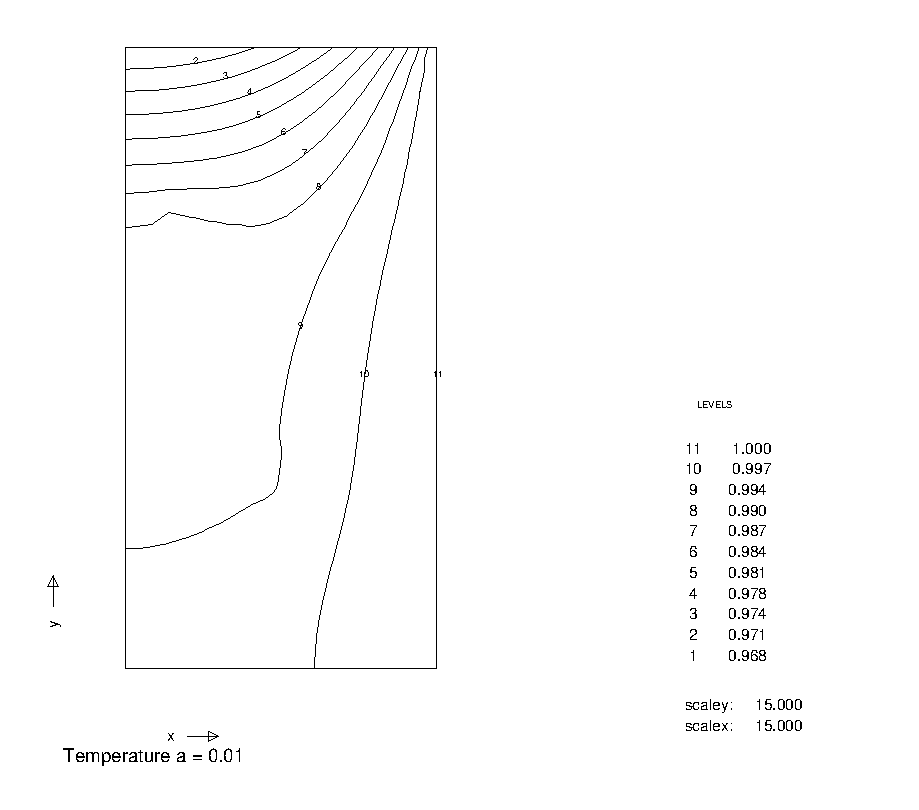
\includegraphics[width=\textwidth]{cont_a001_20el}
                \caption{20 elements contour plot}
                \label{fig:cont_a001_20el}
        \end{subfigure}
        ~
        \begin{subfigure}[b]{0.45\textwidth}
                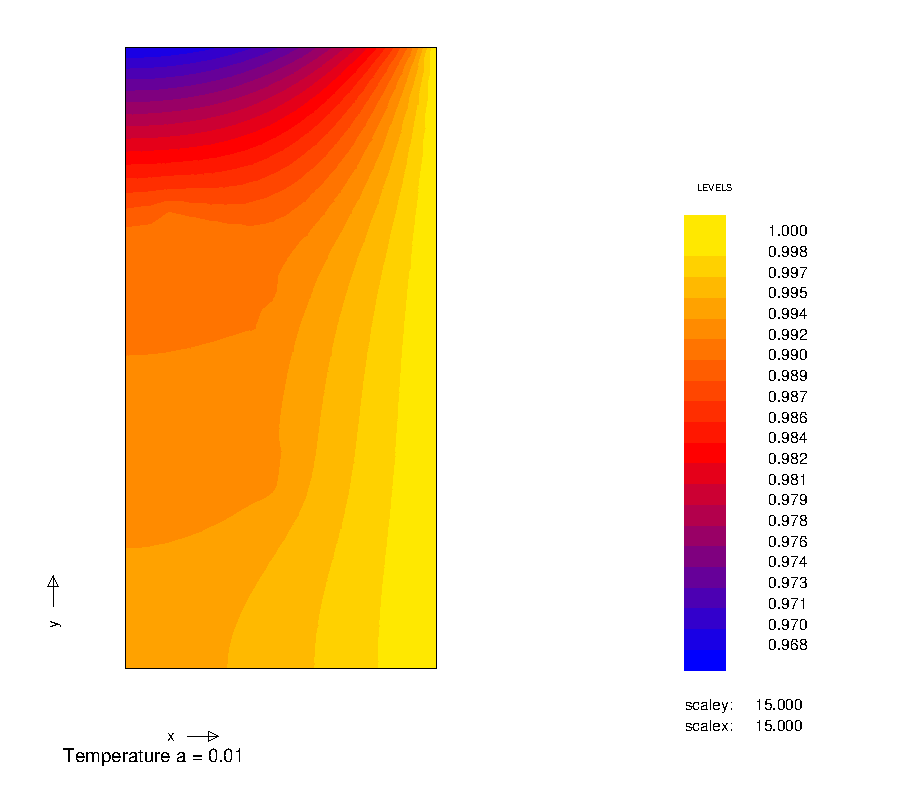
\includegraphics[width=\textwidth]{colplot_a001_20el}
                \caption{20 elements color plot}
                \label{fig:colplot_a001_20el}
        \end{subfigure}
        ~           
        \begin{subfigure}[b]{0.45\textwidth}
                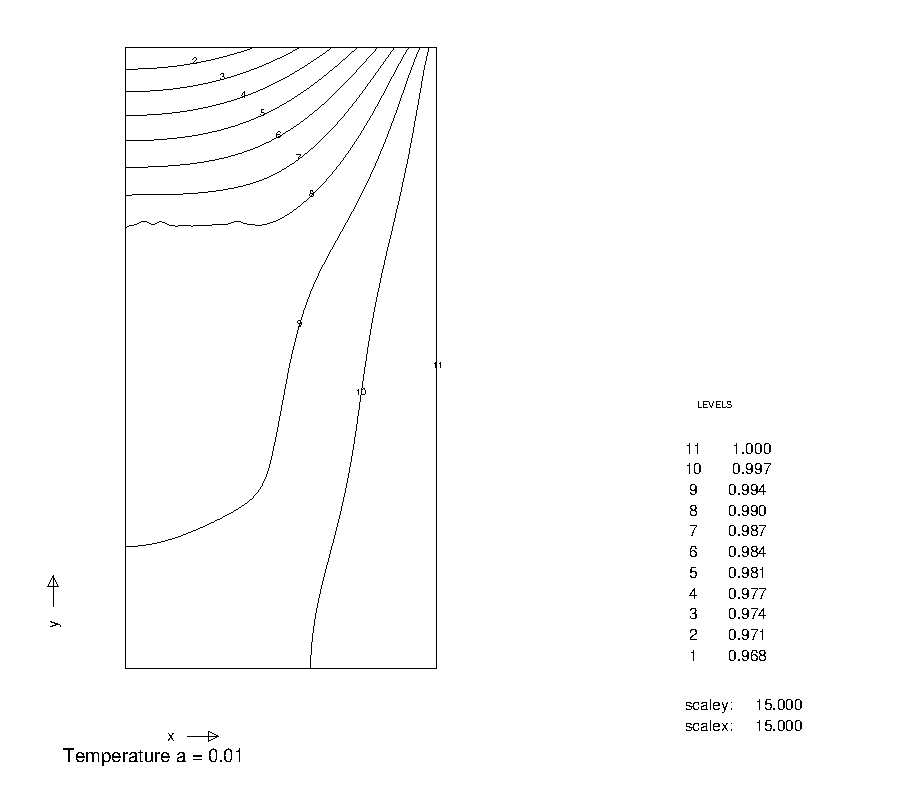
\includegraphics[width=\textwidth]{cont_a001_50el}
                \caption{50 elements contour plot}
                \label{fig:col_a001_50el}
        \end{subfigure}      
        ~
        \begin{subfigure}[b]{0.45\textwidth}
                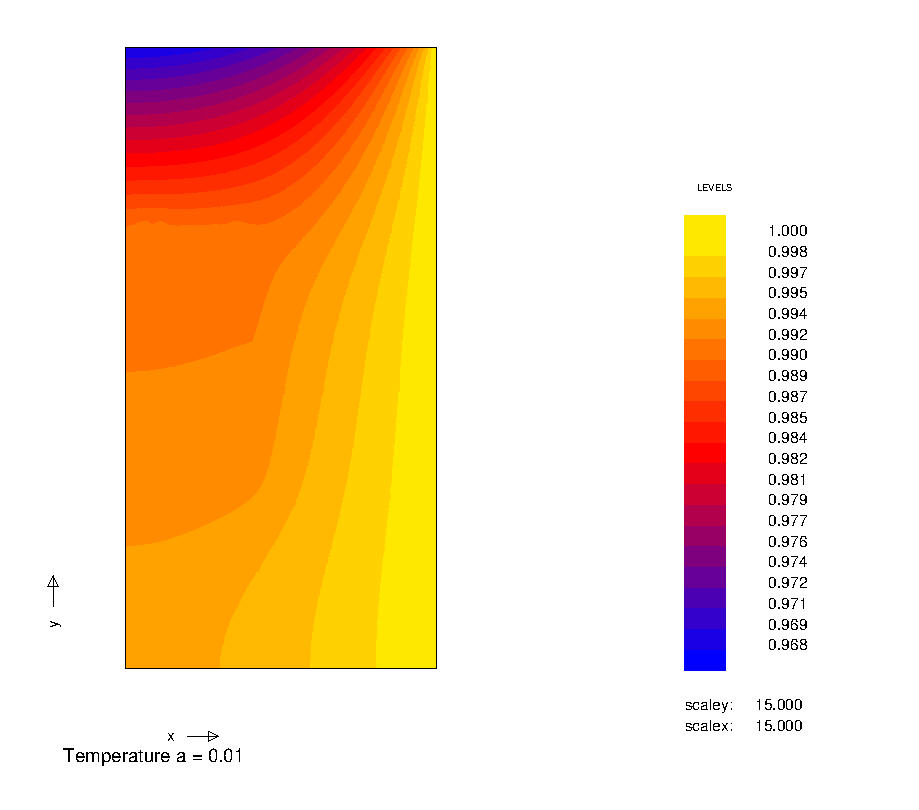
\includegraphics[width=\textwidth]{colplot_a001_50el}
                \caption{20 elements color plot}
                \label{fig:colplot_a001_50el}
        \end{subfigure}
        ~
        \begin{subfigure}[b]{0.45\textwidth}
                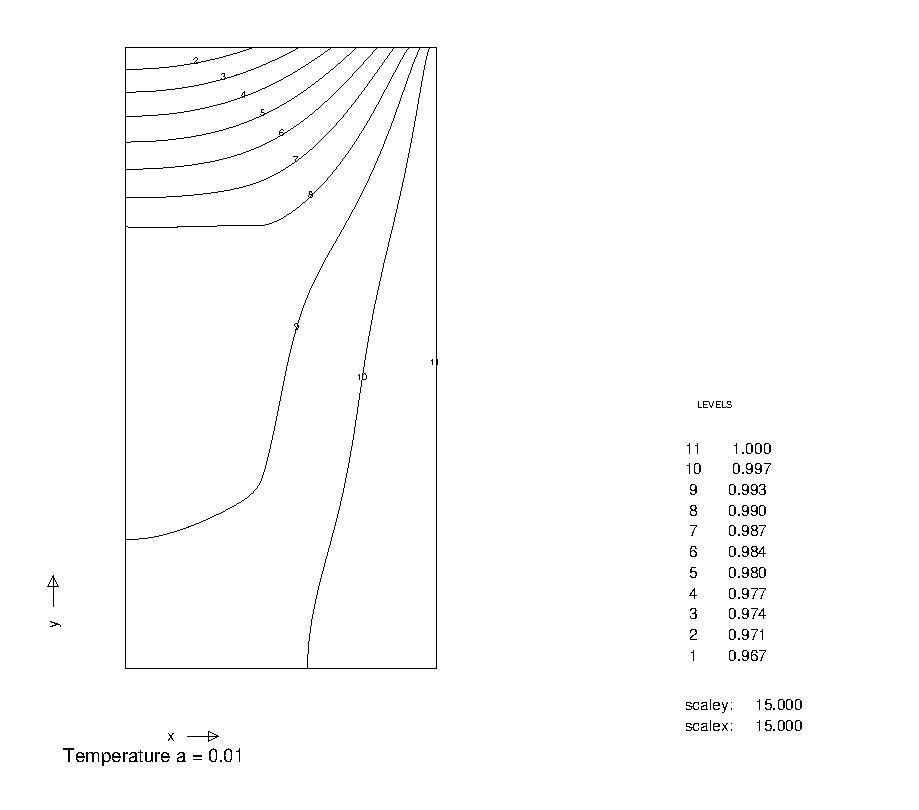
\includegraphics[width=\textwidth]{cont_a001_99el}
                \caption{99 elements contour plot}
                \label{fig:cont_a001_99el}
        \end{subfigure}
        ~ 
        \begin{subfigure}[b]{0.45\textwidth}
                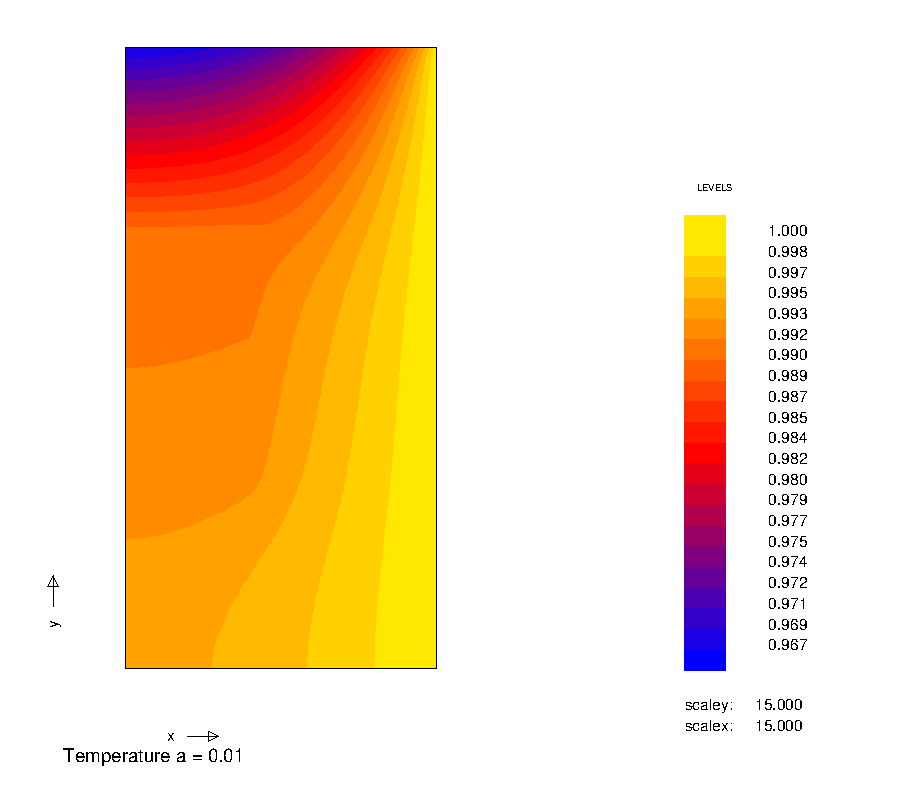
\includegraphics[width=\textwidth]{colplot_a001_99el}
                \caption{99 elements color plot}
                \label{fig:colplot_a001_99el}
        \end{subfigure}
        \caption{solution of the heat equation for a number of elements with $\alpha = 0.01$} 
        \label{fig:10}                                
\end{figure}
\section{Appendix}
%codecodecode
\end{document}
